\section{Introduction}\label{sec:intro}

ZX-diagrams~\cite{CoeckeDuncan2011} are built from spiders, like $\spider{\alpha}$ and $\spider[X]{\beta}$.
Two spiders of the same colour fuse, adding their phases:
\begin{equation}\label{eq:fusion}
  \tikzfig{spider-fusion-Z}
\end{equation}
Spiders of different colours satisfy the bialgebra rule:
\begin{equation}\label{eq:bialgebra}
  \tikzfig{bialgebra-rule}
\end{equation}

Plain TikZ works too, also outside of the figures made with TikZiT, as in Figure~\ref{fig:circuit}.
\begin{figure}[ht]
  \centering
  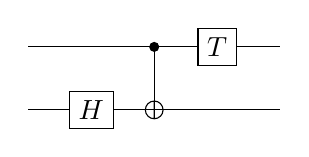
\begin{tikzpicture}[scale=0.8]
    \draw (0,0) -- (4,0) (0,1) -- (4,1);
    \draw (2,0) -- (2,1);
    \filldraw (2,1) circle (2pt);
    \draw (2,0) circle (4pt) (2,-0.14) -- (2,0.14);
    \node[draw, fill=white] at (1,0) {$H$};
    \node[draw, fill=white] at (3,1) {$T$};
  \end{tikzpicture}
  \caption{A circuit drawn with plain TikZ. Inline: \tikz[baseline=-0.6ex]{\draw (0,0) circle (3pt);}.}
  \label{fig:circuit}
\end{figure}
